\documentclass[11pt]{article}
\usepackage{lipsum}
\usepackage[letterpaper, landscape, twocolumn, left=0.5in, right=0.5in, top=1.25in, bottom=0.75in, headheight=0.6in]{geometry} % controls page layout
\usepackage{fancyhdr} % controls headers and footers
\usepackage{lastpage} % enables # of ##
\usepackage{graphicx} % graphics
\usepackage{grffile} % enables multiple periods in file name of \includegraphics
\usepackage{amsmath}  % extended mathematics
\usepackage{booktabs} % book-quality tables
\usepackage{units}    % non-stacked fractions and better unit spacing
\usepackage[T1]{fontenc} % 8-bit encoding of fonts (glyphs are a part of fonts)
% \usepackage{siunitx} % table alignment

\fancypagestyle{title}{ % defining header style for the first page
  \fancyhead[C,R]{}
  \fancyhead[L]{\begin{tabular}{ll}
  \raisebox{-.47\height}{
\includegraphics[height=0.75in, trim=0 -0.1in 0 0]{common/SCE_logo}} &
  \textsc{\textbf{\Huge Customer Report for: E8AQBZ}}
  \end{tabular}}`
  \fancyfoot[L]{\today}
  \fancyfoot[C]{}
  \fancyfoot[R]{\thepage/\pageref{LastPage}}
}

\fancypagestyle{energy}{ % header style for energy charges
  \fancyhead[L]{\textsc{\textbf{\Huge Energy Charges}}}
  \fancyhead[C]{}
  \fancyhead[R]{\textsc{\textbf{\Huge E8AQBZ}}}
  \fancyfoot[L]{\today}
  \fancyfoot[C]{}
  \fancyfoot[R]{\thepage/\pageref{LastPage}}
}

\fancypagestyle{demand}{ % header style for demand charges
  \fancyhead[L]{\textsc{\textbf{\Huge Demand Charges}}}
  \fancyhead[C]{}
  \fancyhead[R]{\textsc{\textbf{\Huge E8AQBZ}}}
  \fancyfoot[L]{\today}
  \fancyfoot[C]{}
  \fancyfoot[R]{\thepage/\pageref{LastPage}}
}

\renewcommand{\headrulewidth}{0.4pt}
\renewcommand{\footrulewidth}{0.4pt}

\begin{document}
\pagestyle{title}
This report summarizes the time-dependent portion of your electricity charges, the portion of the charges dependent on your usage patterns. It also compares your charges relative to those of others in your ``peer group'' -- those within the same North American Industry (NAICS) code and subscribed to the same time of use rate (TOU). It is provided to you for your information and as a backdrop for the conversation with Southern California Edison (SCE) to find opportunities for savings.

The analysis is performed by back-casting your last year's consumption to the rates currently in effect. As such, it is a forecast of your future payments, not an accurate replica of your earlier ones. 

\vspace{3ex}
\textbf{\Large Components of the Bill}
\vspace{1ex}

The time-dependent part of an electric bill has three main components: energy charges, facility charges, and demand charges. The first component - energy charges - are collected to recover your utility's cost to procure electricity. They are calculated by multiplying your consumption over a given time interval by the price of electricity at the same interval and summing these charges over the billing period (typically a calendar month) The remaining two components are  The makeup of these charges for the year and by month are shown in Figures~\ref{fig:pie} and \ref{fig:bars}, respectively.
\begin{figure}[!h]
\centering
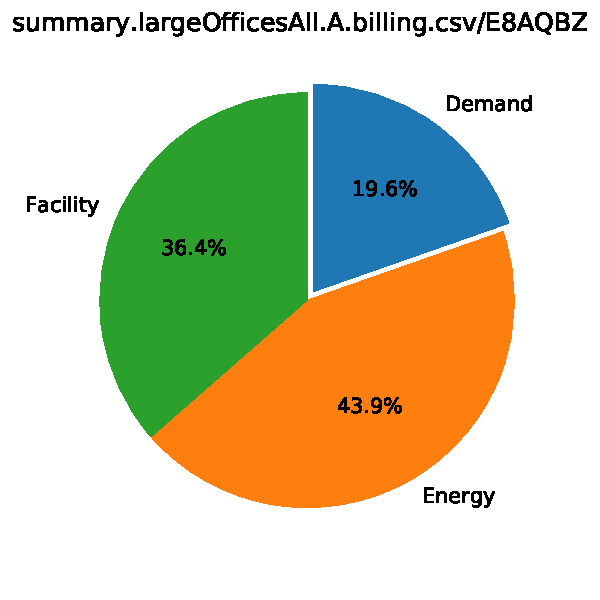
\includegraphics[height=3in, page=1, trim=0in 0.45in 0in 0.45in, clip]{visuals/E8AQBZ.piechart.pdf}
\caption{Makeup of annual charges}
\label{fig:pie}
\end{figure}

\begin{figure}[!h]
\centering
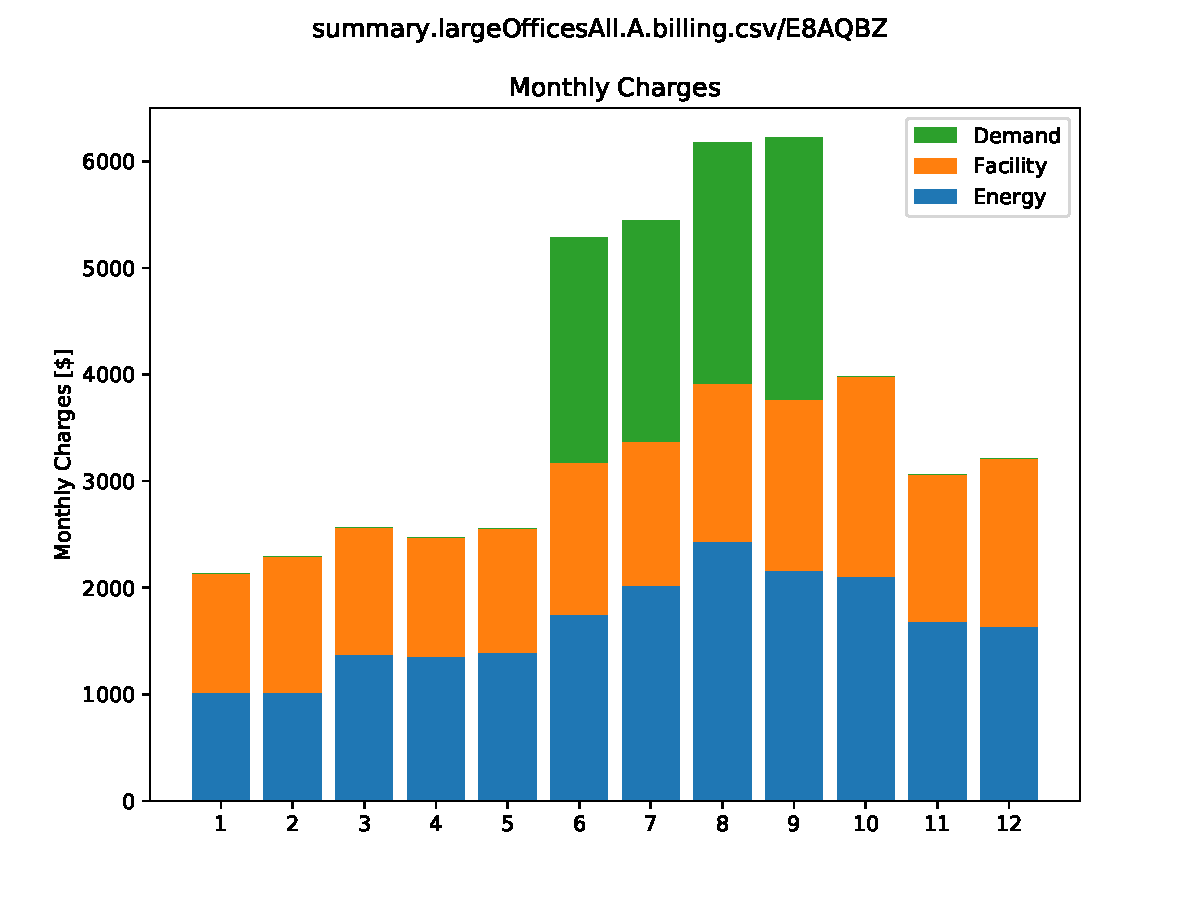
\includegraphics[width=\columnwidth, page=1, trim=0in 0.45in 0in 0.45in, clip]{visuals/E8AQBZ.boxplot.pdf}
\caption{Makeup of monthly charges}
\label{fig:bars}
\end{figure}

Note that the demand charges are collected only in the four summer months, yet they account for 56.1\% of the total annual bill. The expected annual charges by bill component are summarized in Table~\ref{tab:annual}.

\begin{table}[th!]
  \centering
  \caption{Components of Annual Electric Bill}
  \vspace{1.5ex}
  \label{tab:annual}
  \begin{tabular}{lr}
    Bill component & Amount [\$] \\
    \midrule
    Facility & 16551.02 \\
    Energy & 19953.42 \\
    Demand & 8920.06 \\
    \midrule
    Total & 45424.51
  \end{tabular}
\end{table}
\clearpage

\newgeometry{twocolumn, left=0.5in, right=0.5in, top=0.75in, bottom=0.75in, headheight=0.1in}
\pagestyle{energy}

\begin{figure}[!h]
\centering
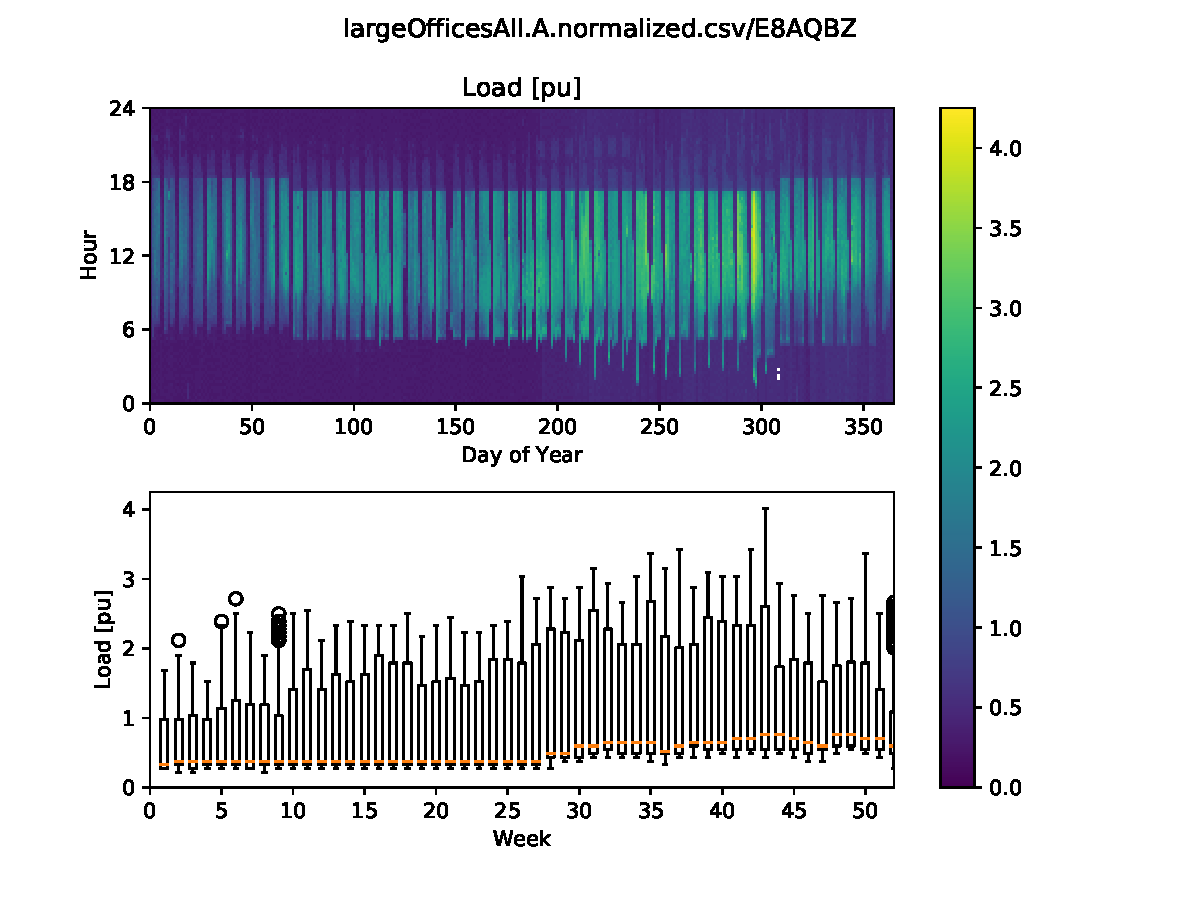
\includegraphics[width=\columnwidth, page=1, trim=0in 0.45in 0in 0.45in, clip]{visuals/E8AQBZ.heatmap.pdf}
\caption{Normalized consumption for E8AQBZ}
\label{fig:heatmap}
\end{figure}

\begin{figure}[!h]
\centering
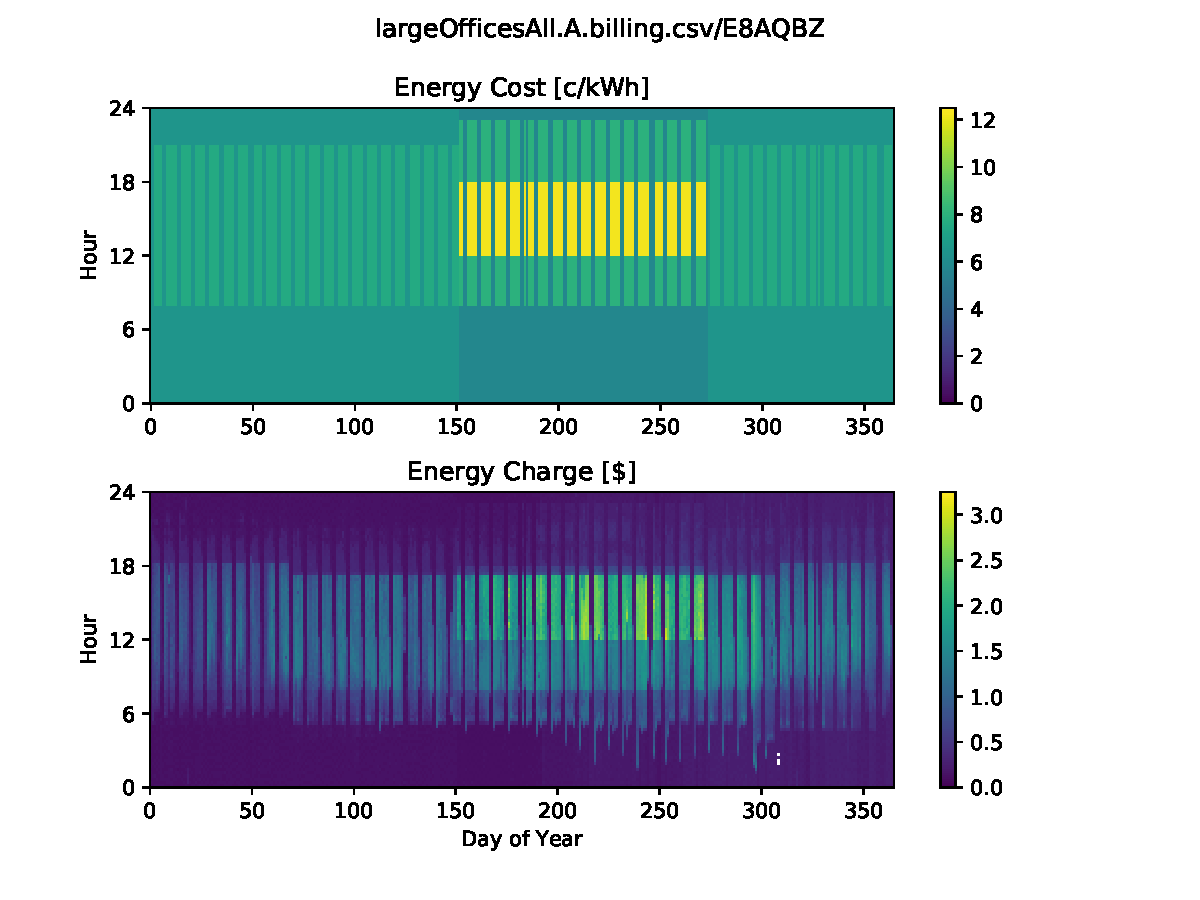
\includegraphics[width=\columnwidth, page=1, trim=0in 3in 0in 0.45in, clip]{visuals/E8AQBZ.billing.Heatmap.pdf}
\caption{Energy price on TOU-GS3-B}
\label{fig:toumap}
\end{figure}

\lipsum[1][1-7]

\begin{table}[th!]
  \centering
  \caption{Monthly Energy Charges}
  \vspace{1.5ex}
  \label{tab:energy}
  \begin{tabular}{p{0.75in}rp{0.2in}p{0.75in}r}
    Month & Charge [\$] & & Month & Charge [\$] \\
    \midrule
    Jan & 1019.21 & & Jul & 2023.68 \\
    Feb & 1018.19 & & Aug & 2438.58 \\
    Mar & 1372.18 & & Sep & 2160.32 \\
    Apr & 1355.80 & & Oct & 2103.42 \\
    Jun & 1746.72 & & Nov & 1685.89 \\
    May & 1389.79 & & Dec & 1639.64 \\
    \midrule
    Average & 1662.78 & & &
  \end{tabular}
\end{table}

\vspace{3ex}
\textbf{\Large Peer performance}
\vspace{1ex}

\lipsum[1][1-7]

\begin{figure}[!h]
\centering
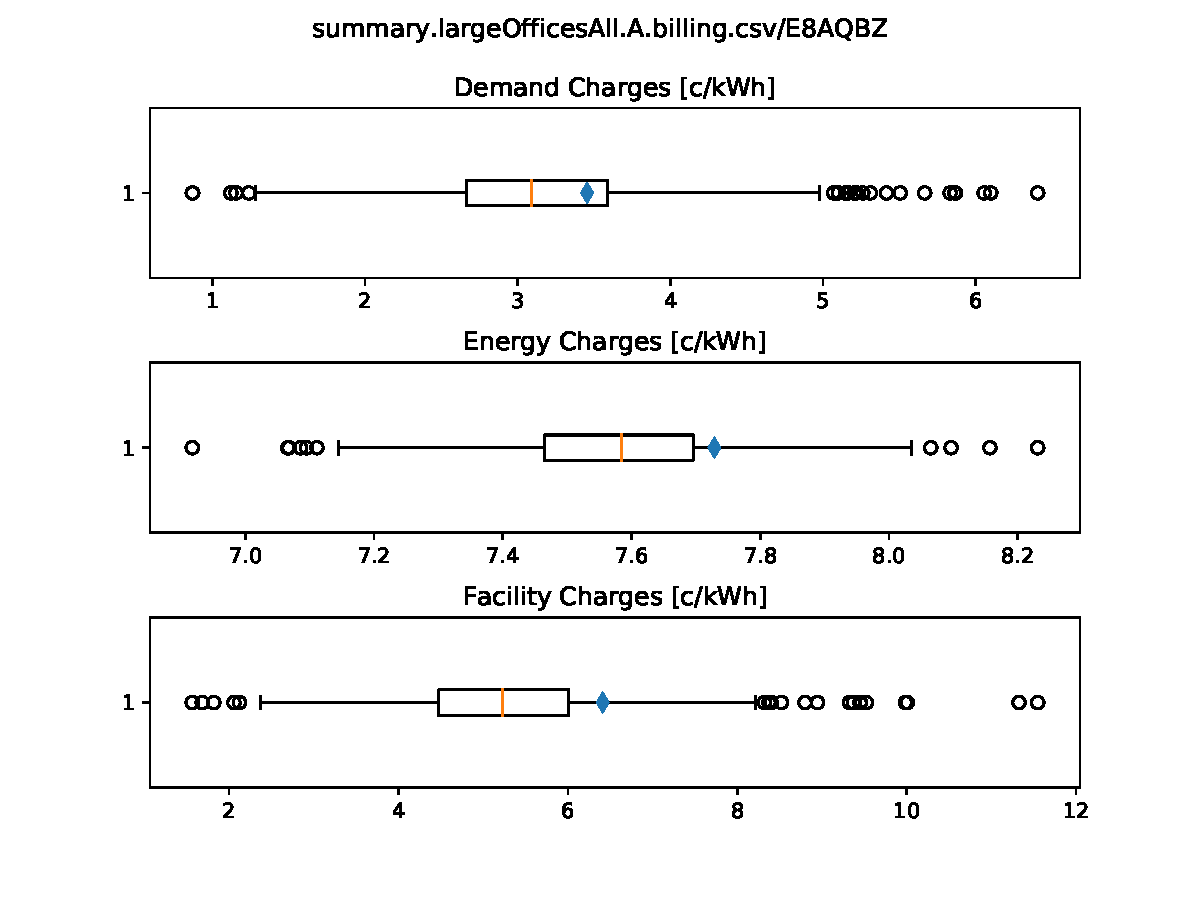
\includegraphics[width=\columnwidth, page=1, trim=0in 2.1in 0in 2.1in, clip]{visuals/E8AQBZ.whiskerchart.pdf}
\caption{Average annual energy price for E8AQBZ compared to peers}
\label{fig:PeerCompEn}
\end{figure}

\clearpage

\newgeometry{twocolumn, left=0.5in, right=0.5in, top=0.75in, bottom=0.75in, headheight=0.1in}
\pagestyle{demand}
\lipsum[1][1-7]

\begin{figure}[!h]
\centering
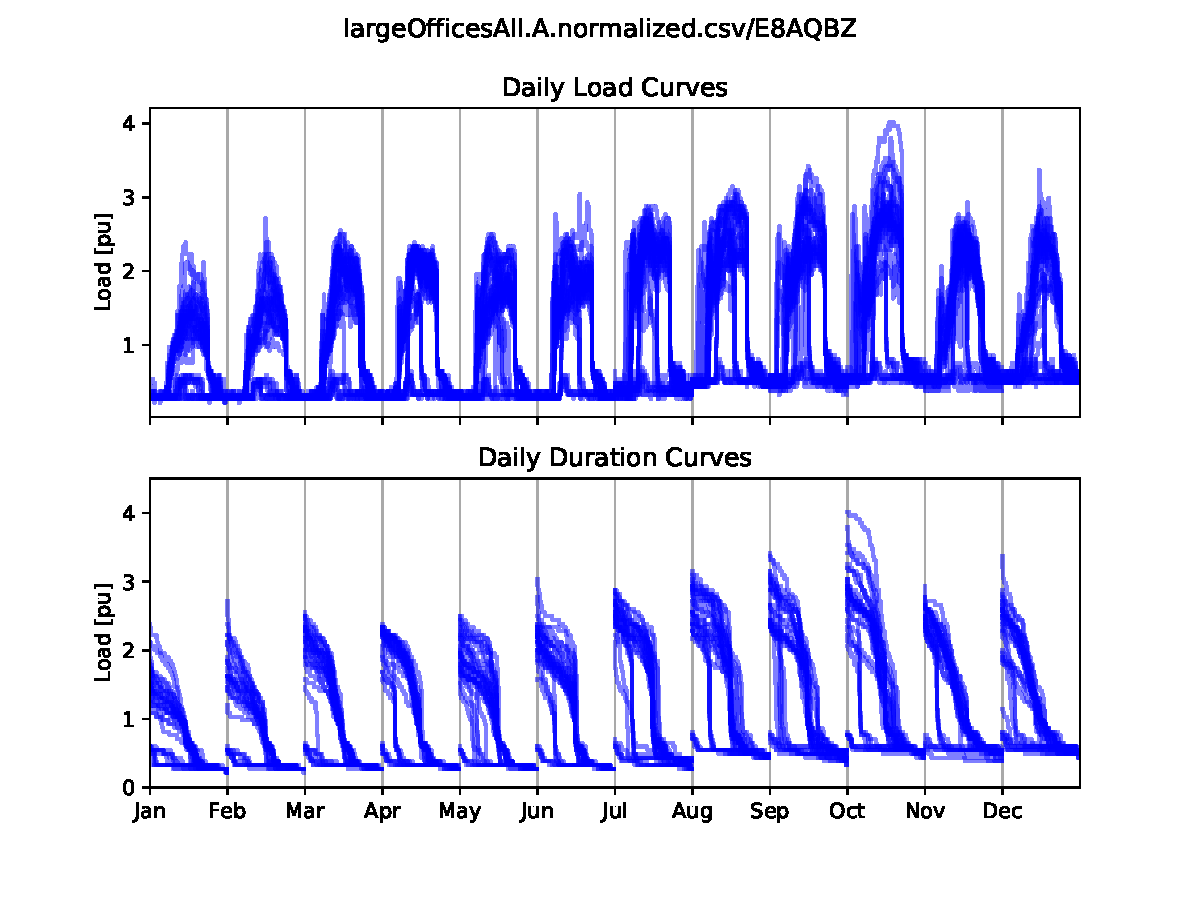
\includegraphics[width=\columnwidth, page=1, trim=0in 0.45in 0in 0.45in, clip]{visuals/E8AQBZ.duration.monthly.test.pdf}
\caption{Normalized load and demand profiles for E8AQBZ}
\label{fig:duration}
\end{figure}

\lipsum[1][1-7]

\begin{table}[th!]
  \centering
  \caption{Monthly Demand Charges}
  \vspace{1.5ex}
  \label{tab:demand}
  \begin{tabular}{p{0.75in}rp{0.2in}p{0.75in}r}
    Month & Charge [\$] & & Month & Charge [\$] \\
    \midrule
    Jan & 1118.66 & & Jul & 3420.97 \\
    Feb & 1271.20 & & Aug & 3741.74 \\
    Mar & 1194.93 & & Sep & 4062.51 \\
    Apr & 1118.66 & & Oct & 1881.38 \\
    May & 1169.50 & & Nov & 1372.90 \\
    Jun & 3542.35 & & Dec & 1576.29 \\
    \midrule
    Average & 2122.59
  \end{tabular}
\end{table}

\vspace{3ex}
\textbf{\Large Peer performance}
\vspace{1ex}

\lipsum[1][1-7]

\begin{figure}[!h]
\centering
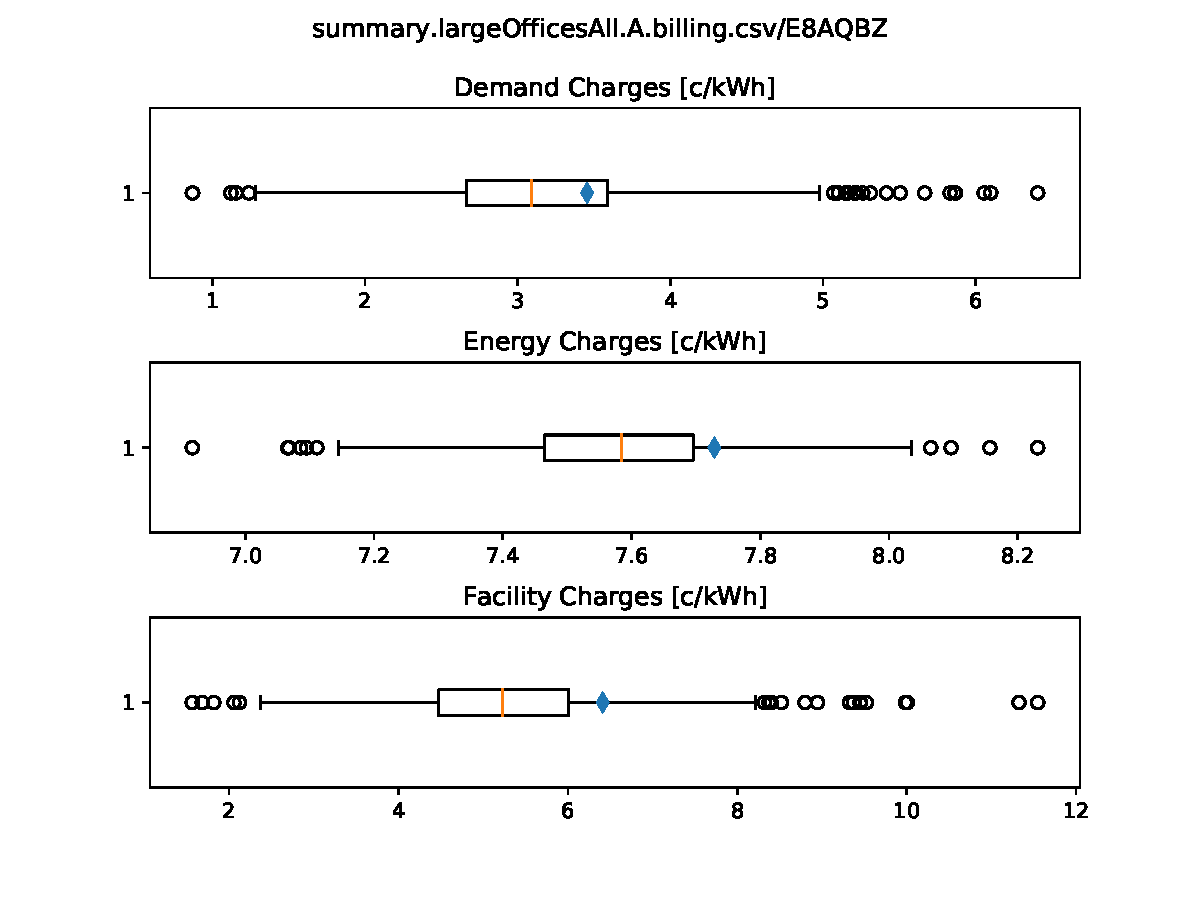
\includegraphics[width=\columnwidth, page=1, trim=0in 3.8in 0in 0.5in, clip]{visuals/E8AQBZ.whiskerchart.pdf}
\caption{Average annual demand price for E8AQBZ compared to peers}
\label{fig:PeerCompDmnd}
\end{figure}

\end{document}
